\documentclass{ctexart}
\usepackage{graphicx}
\usepackage{hyperref}

\graphicspath{{figures/}}

\hypersetup{
    colorlinks=true,
    linkcolor=blue,
    filecolor=blue,
    urlcolor=blue,
    citecolor=cyan,
}


\begin{document}
    % 导言区:\usepackage{graphicx}
    % 语法:\includegraphics[<选项>]{文件名}
    % 支持格式:EPS, PDF, PNG, JPEG, BMP
    
    \LaTeX{}中的插图:

    
\includegraphics{lion.eps}
    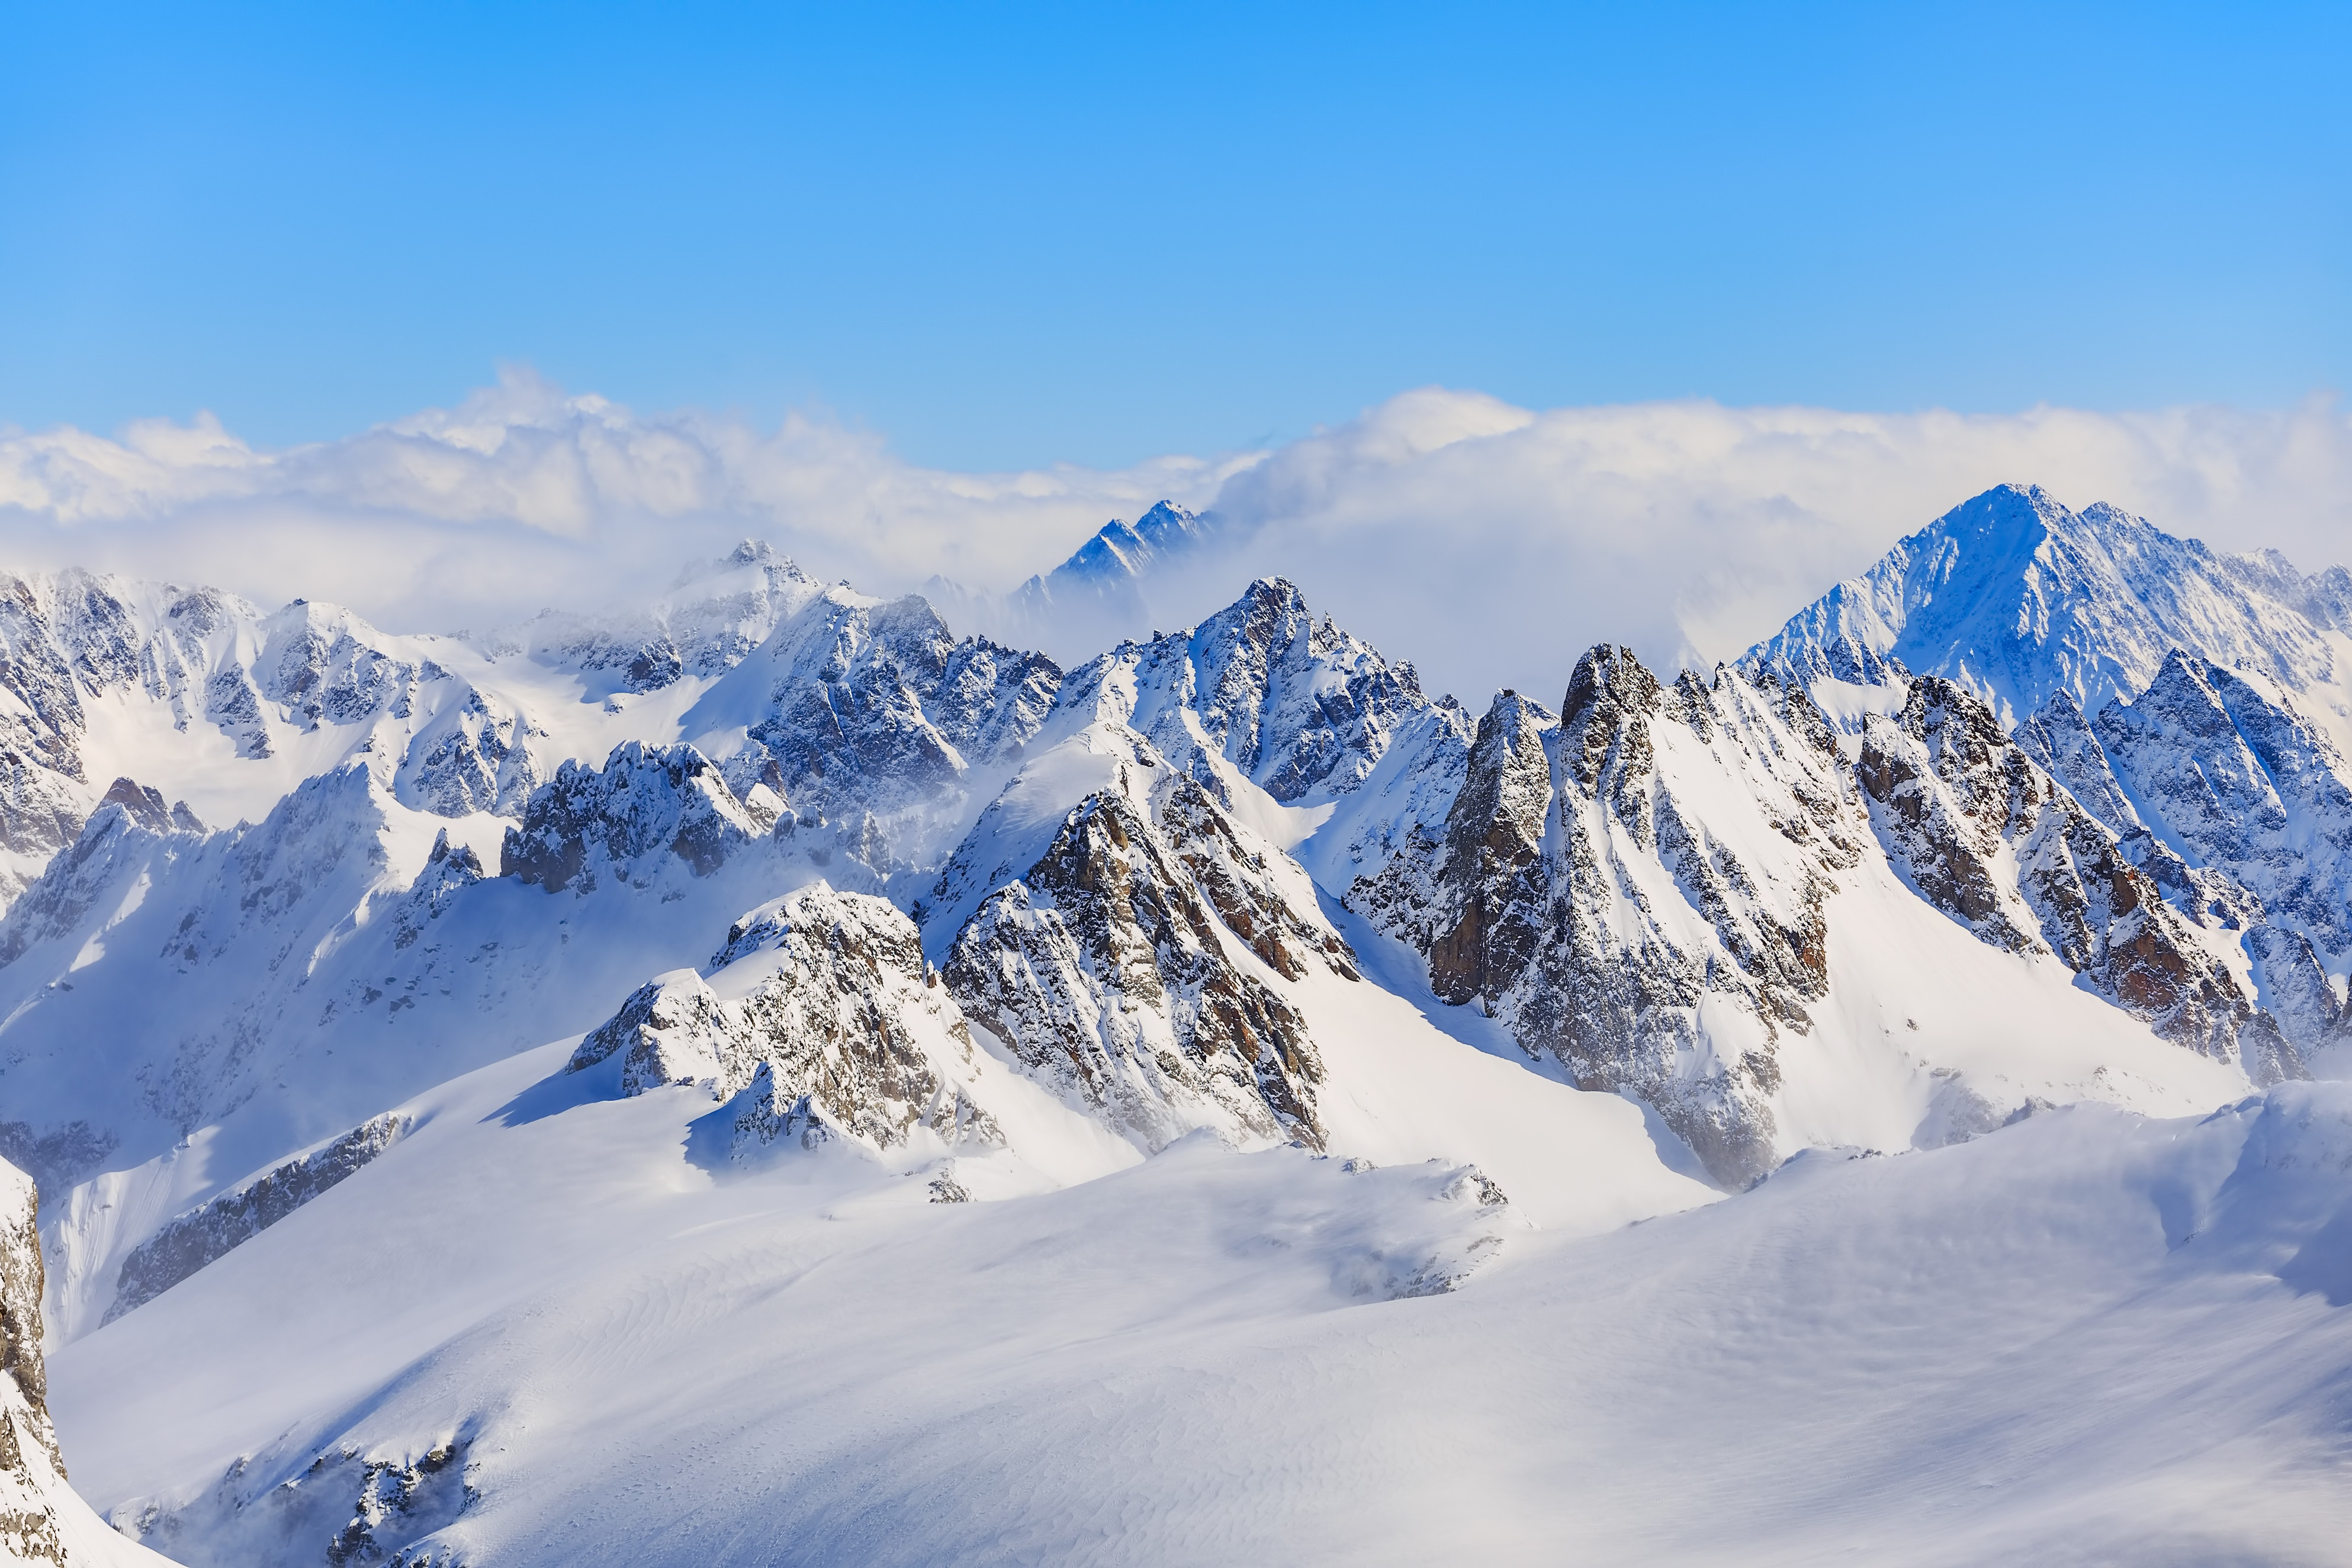
\includegraphics{mountain.jpg}
    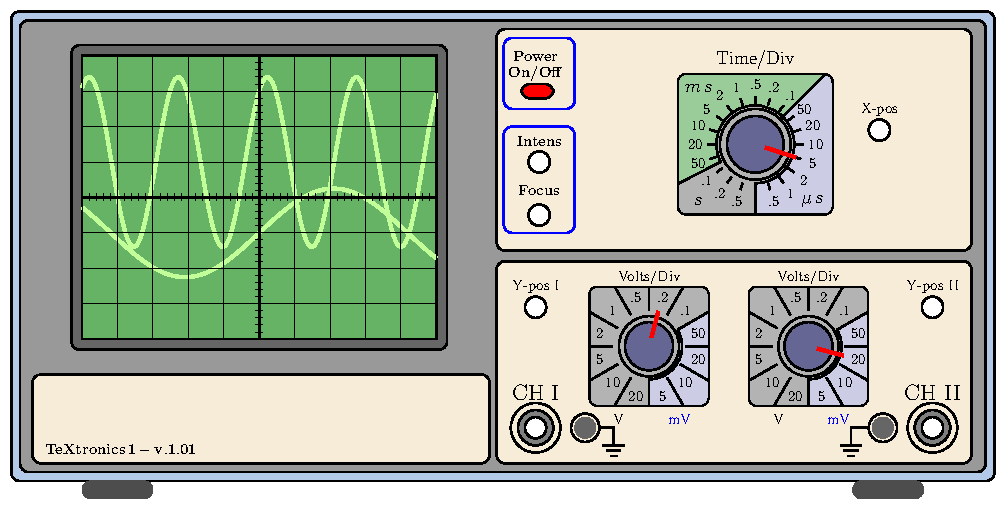
\includegraphics{oscilloscope.pdf}

    
\includegraphics[scale=0.3]{lion}
    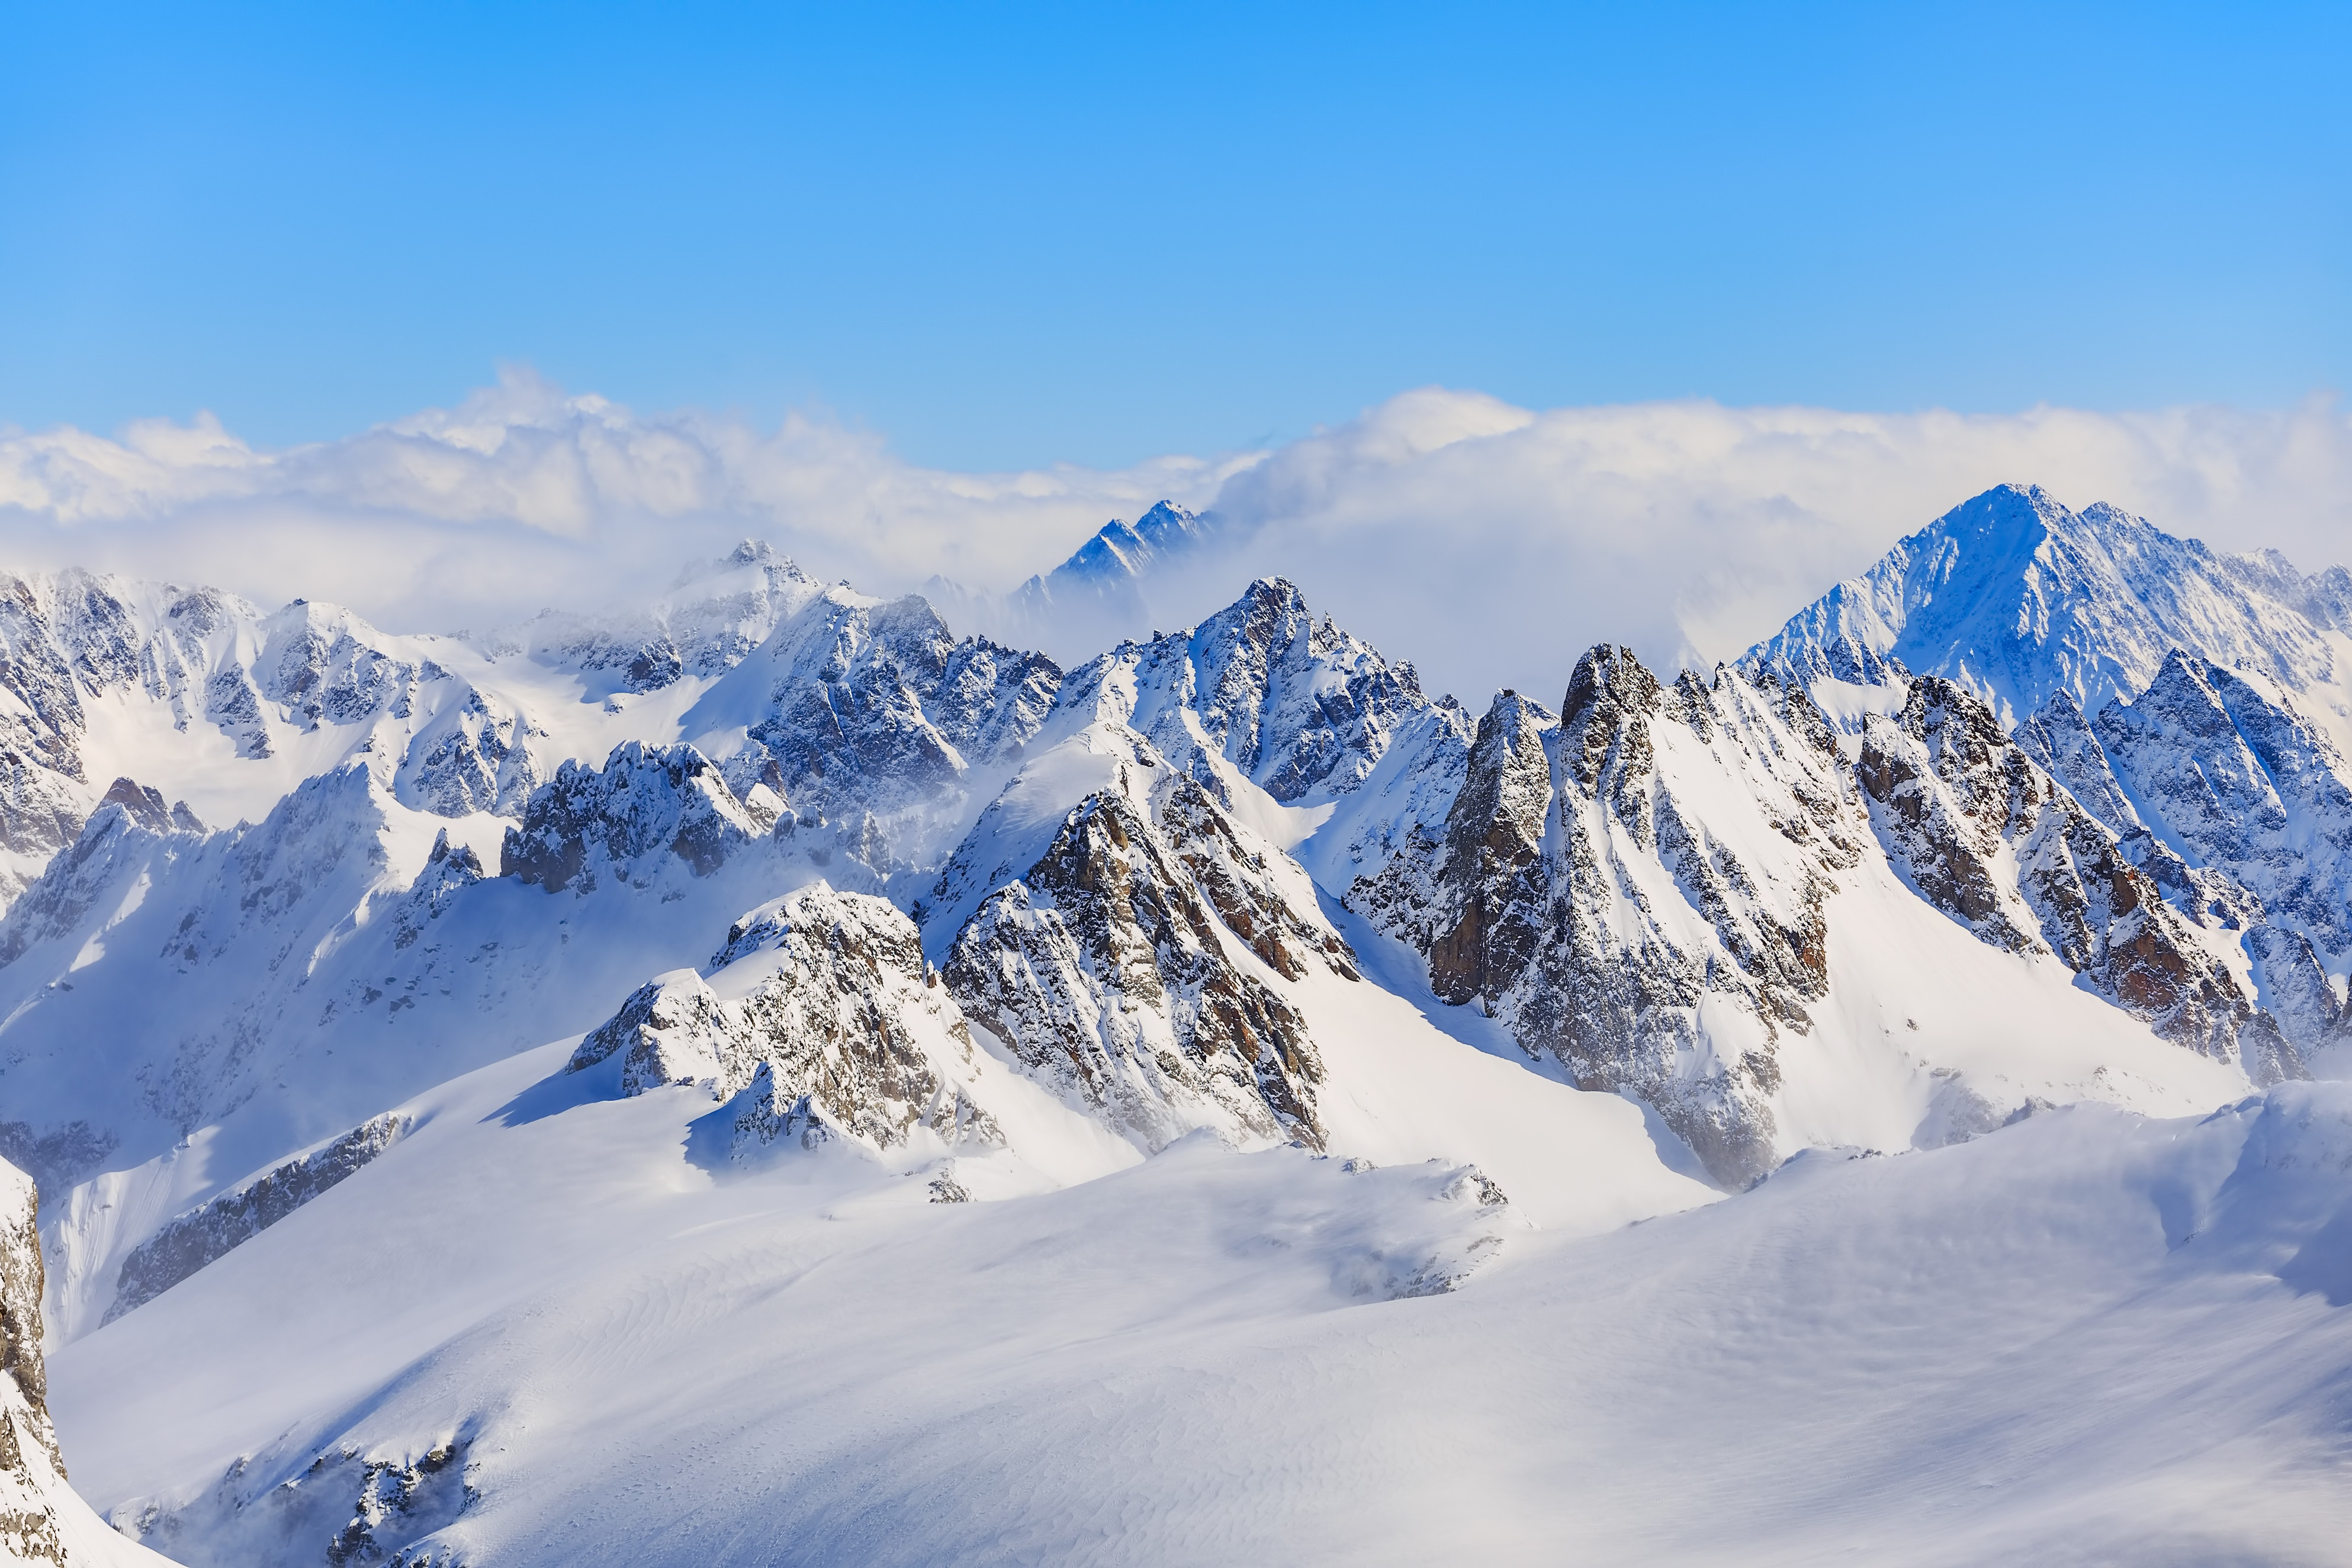
\includegraphics[scale=0.03]{mountain}
    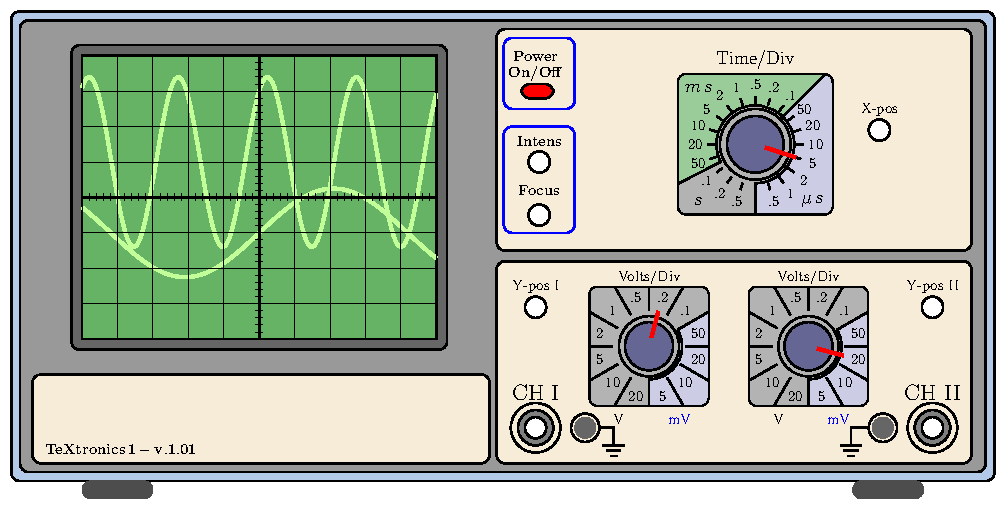
\includegraphics[scale=0.3]{oscilloscope}
    
    
\includegraphics[height=2cm]{lion}
    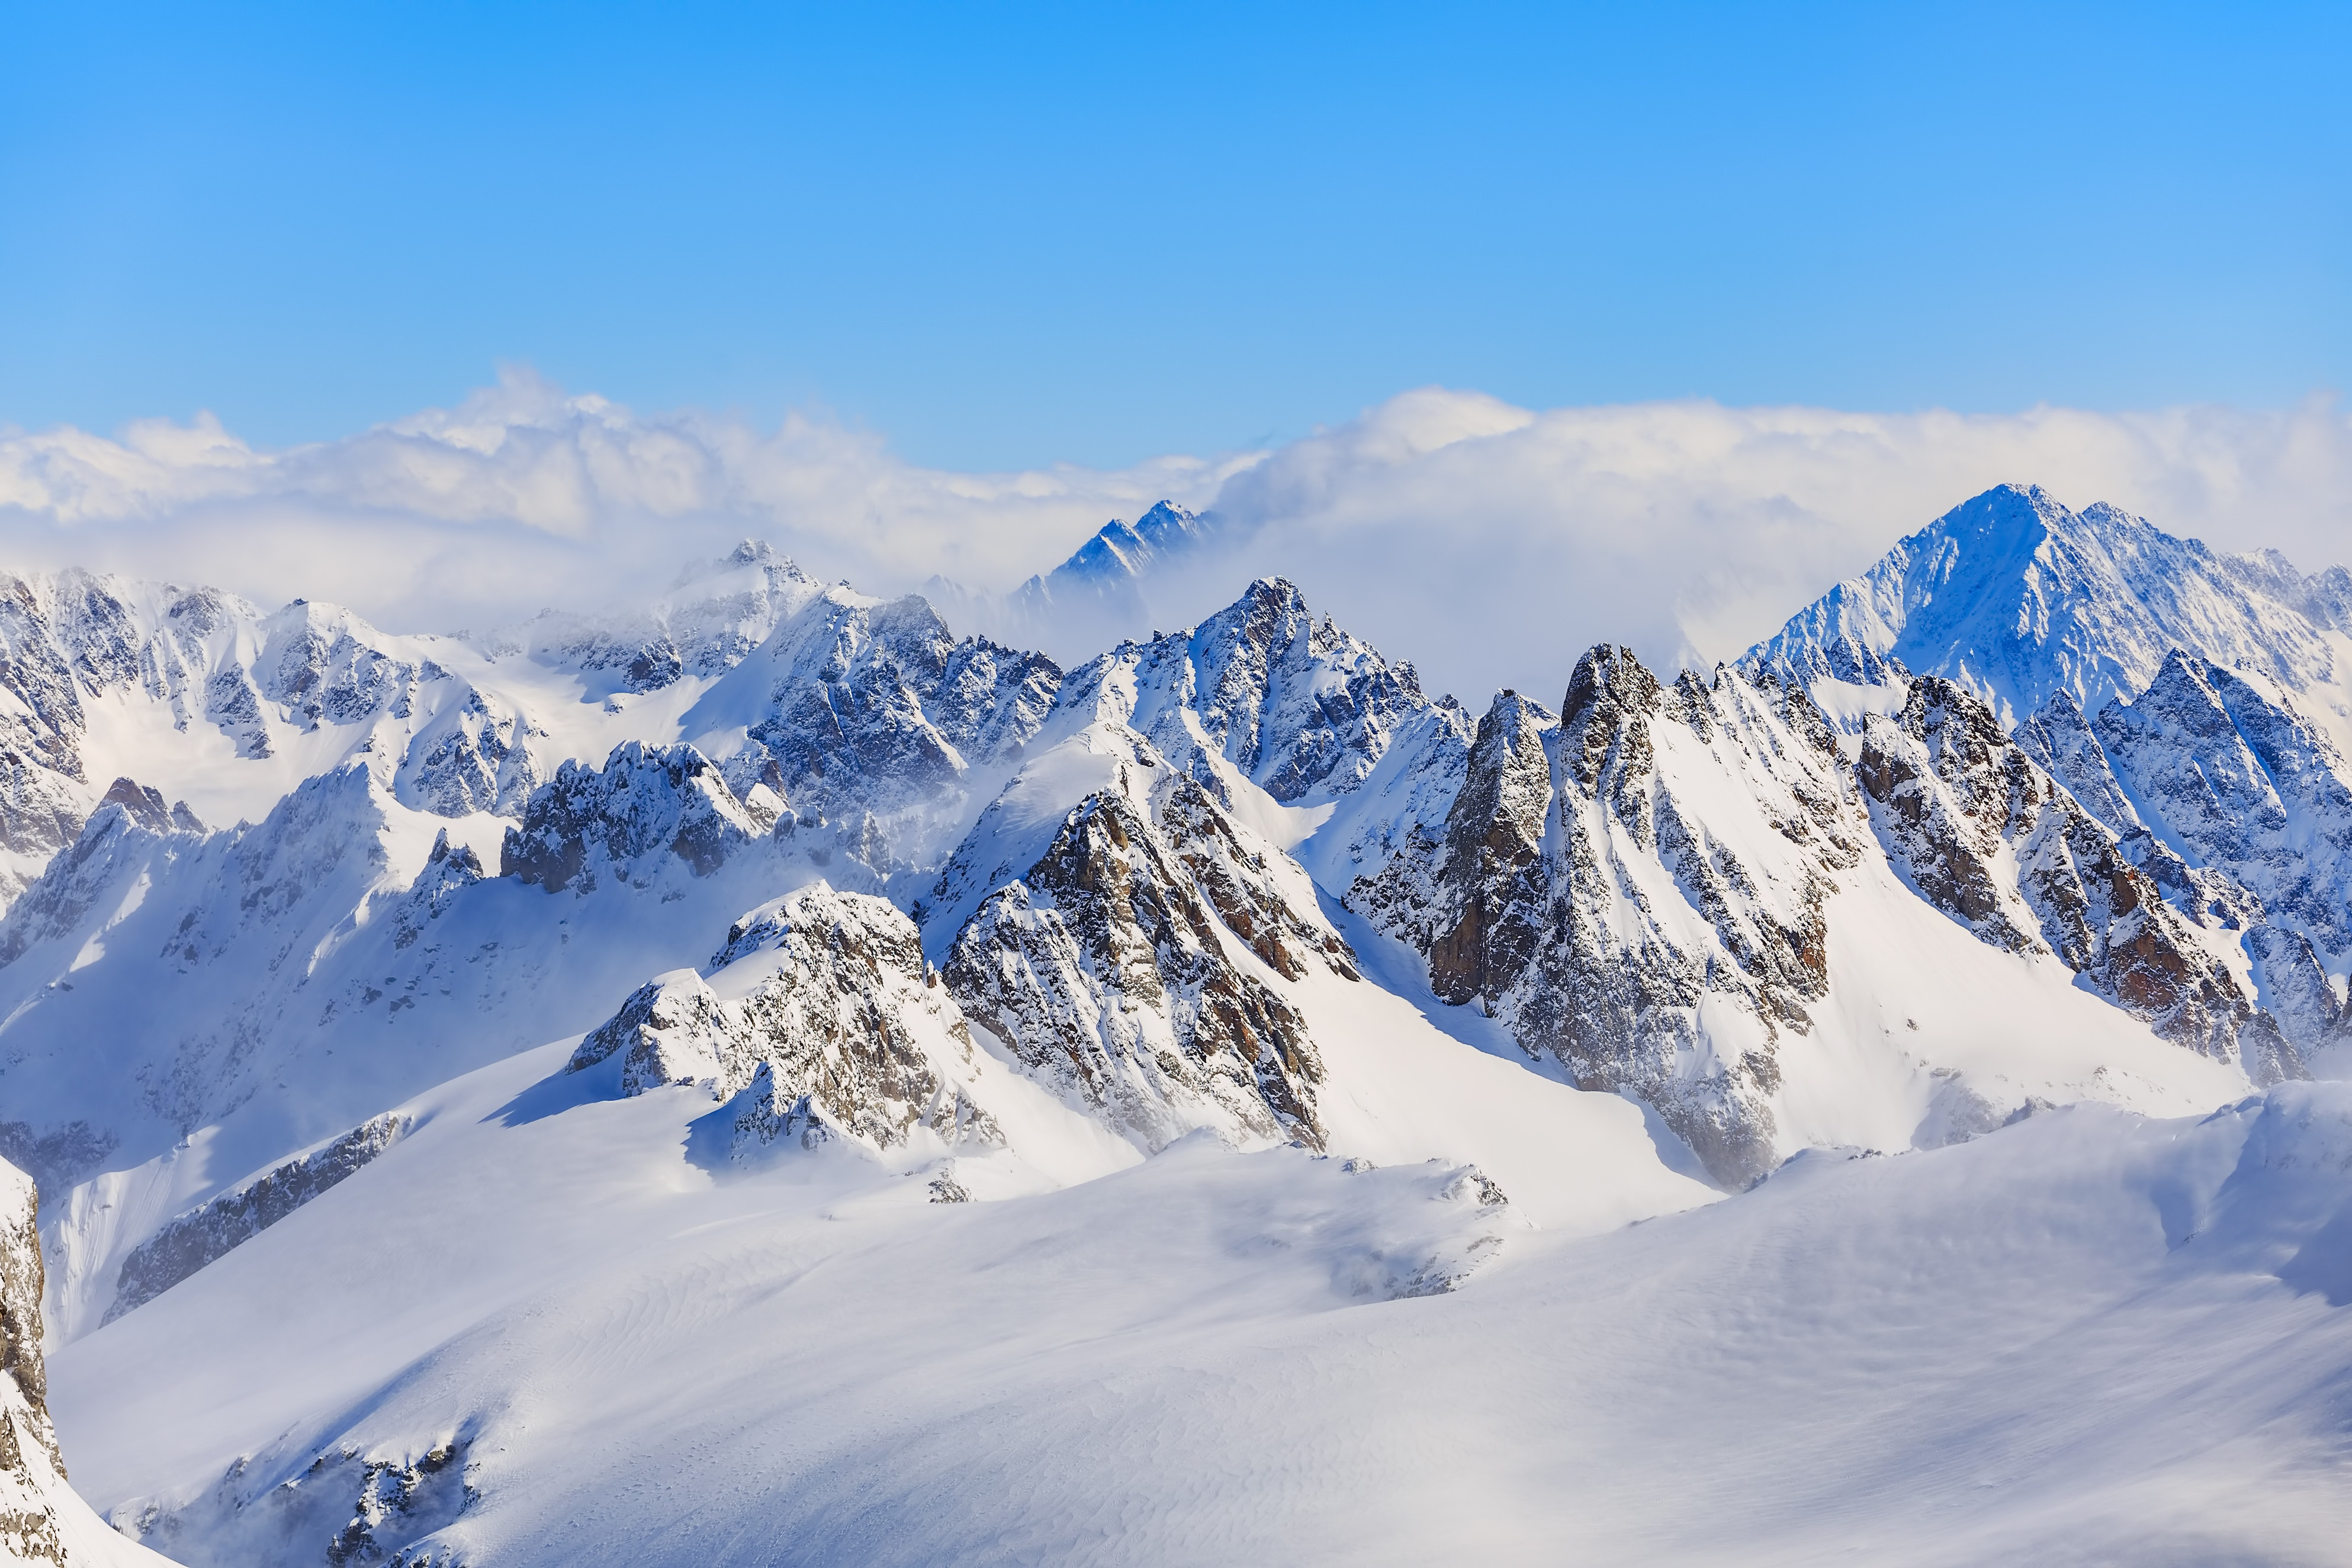
\includegraphics[height=2cm]{mountain}
    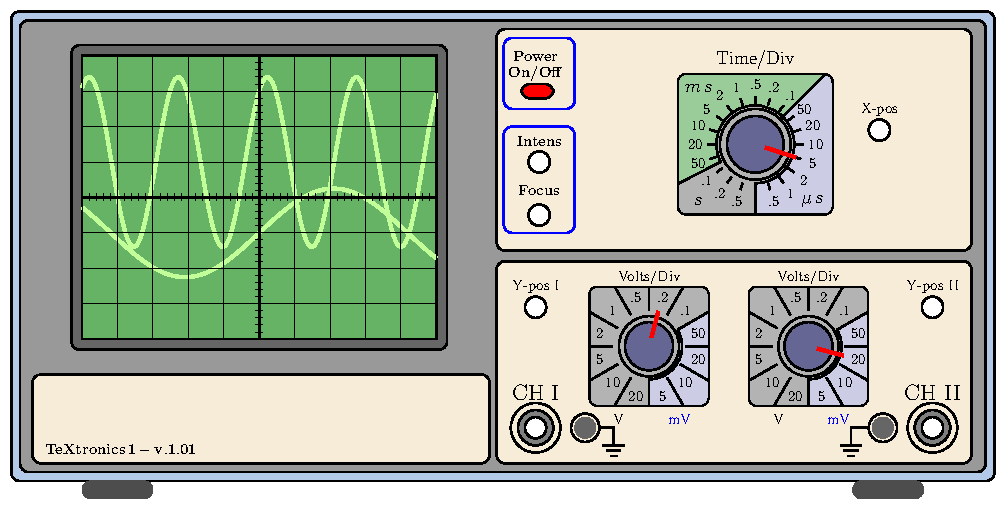
\includegraphics[height=2cm]{oscilloscope}

    
\includegraphics[width=2cm]{lion}
    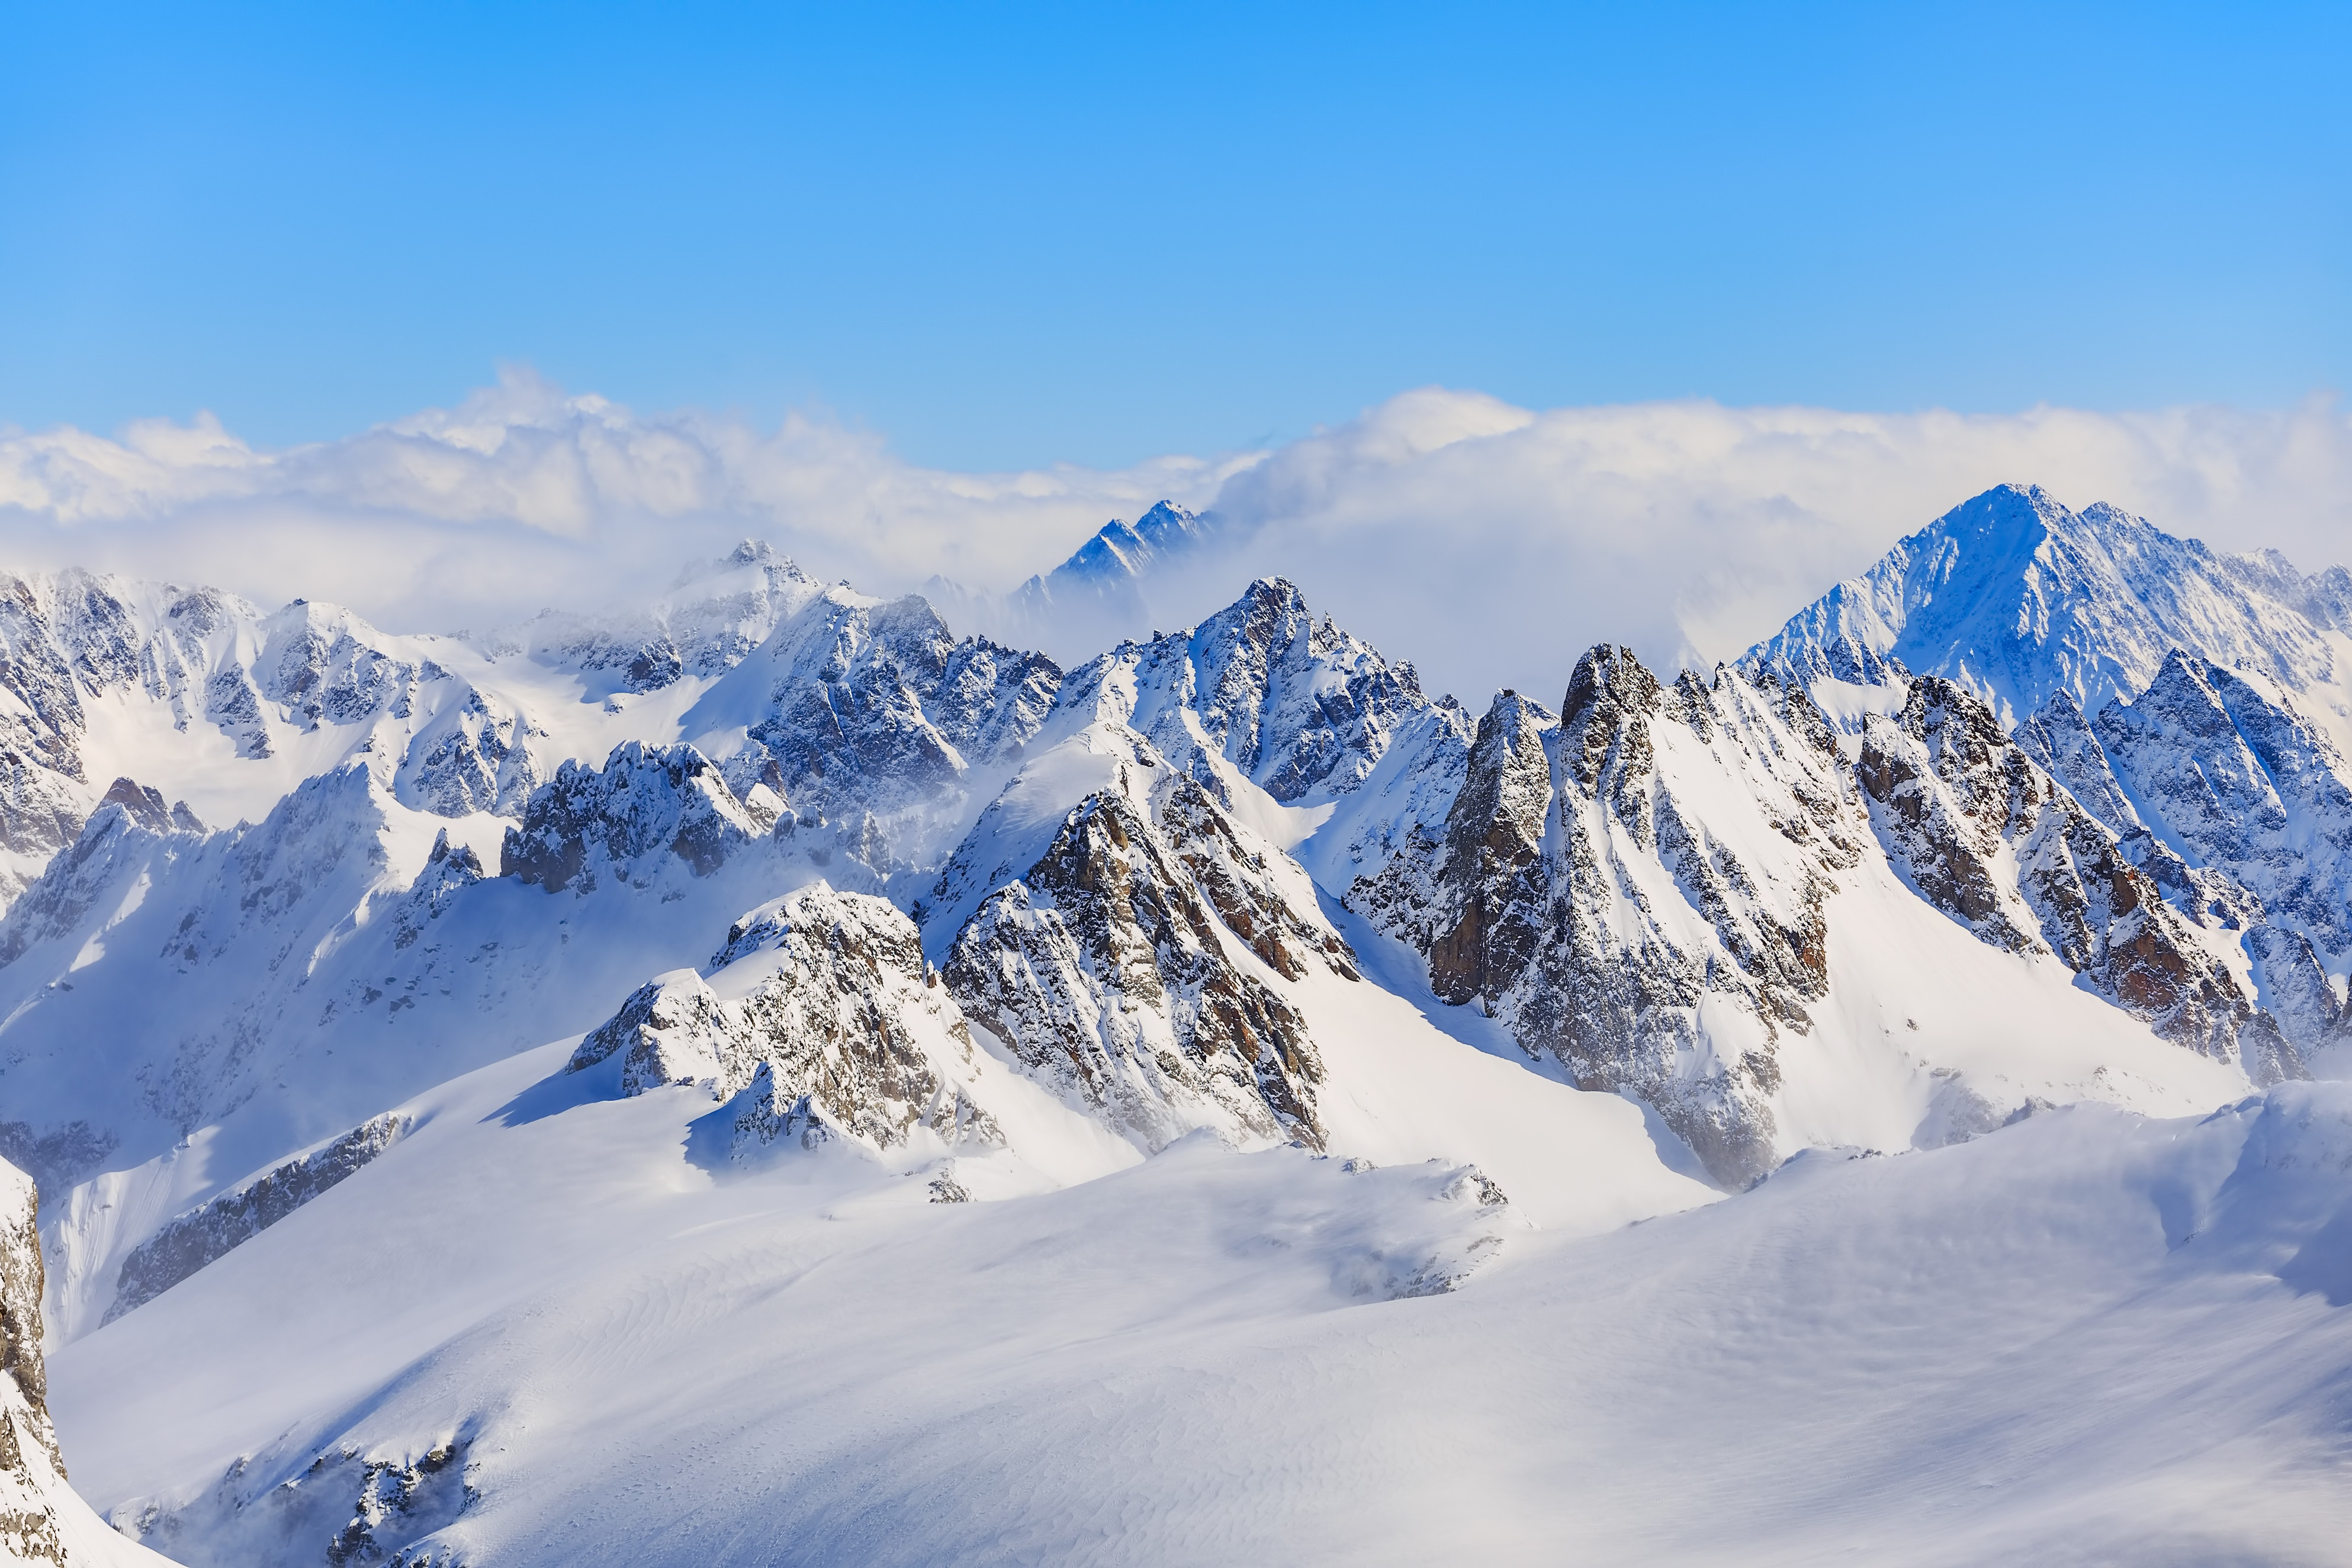
\includegraphics[width=2cm]{mountain}
    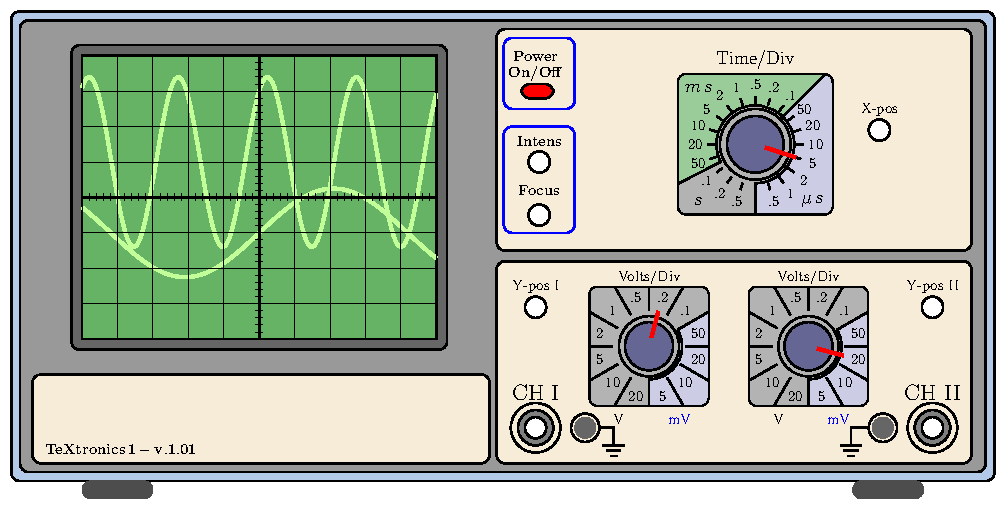
\includegraphics[width=2cm]{oscilloscope}

    
\includegraphics[height=0.1\textheight]{lion}
    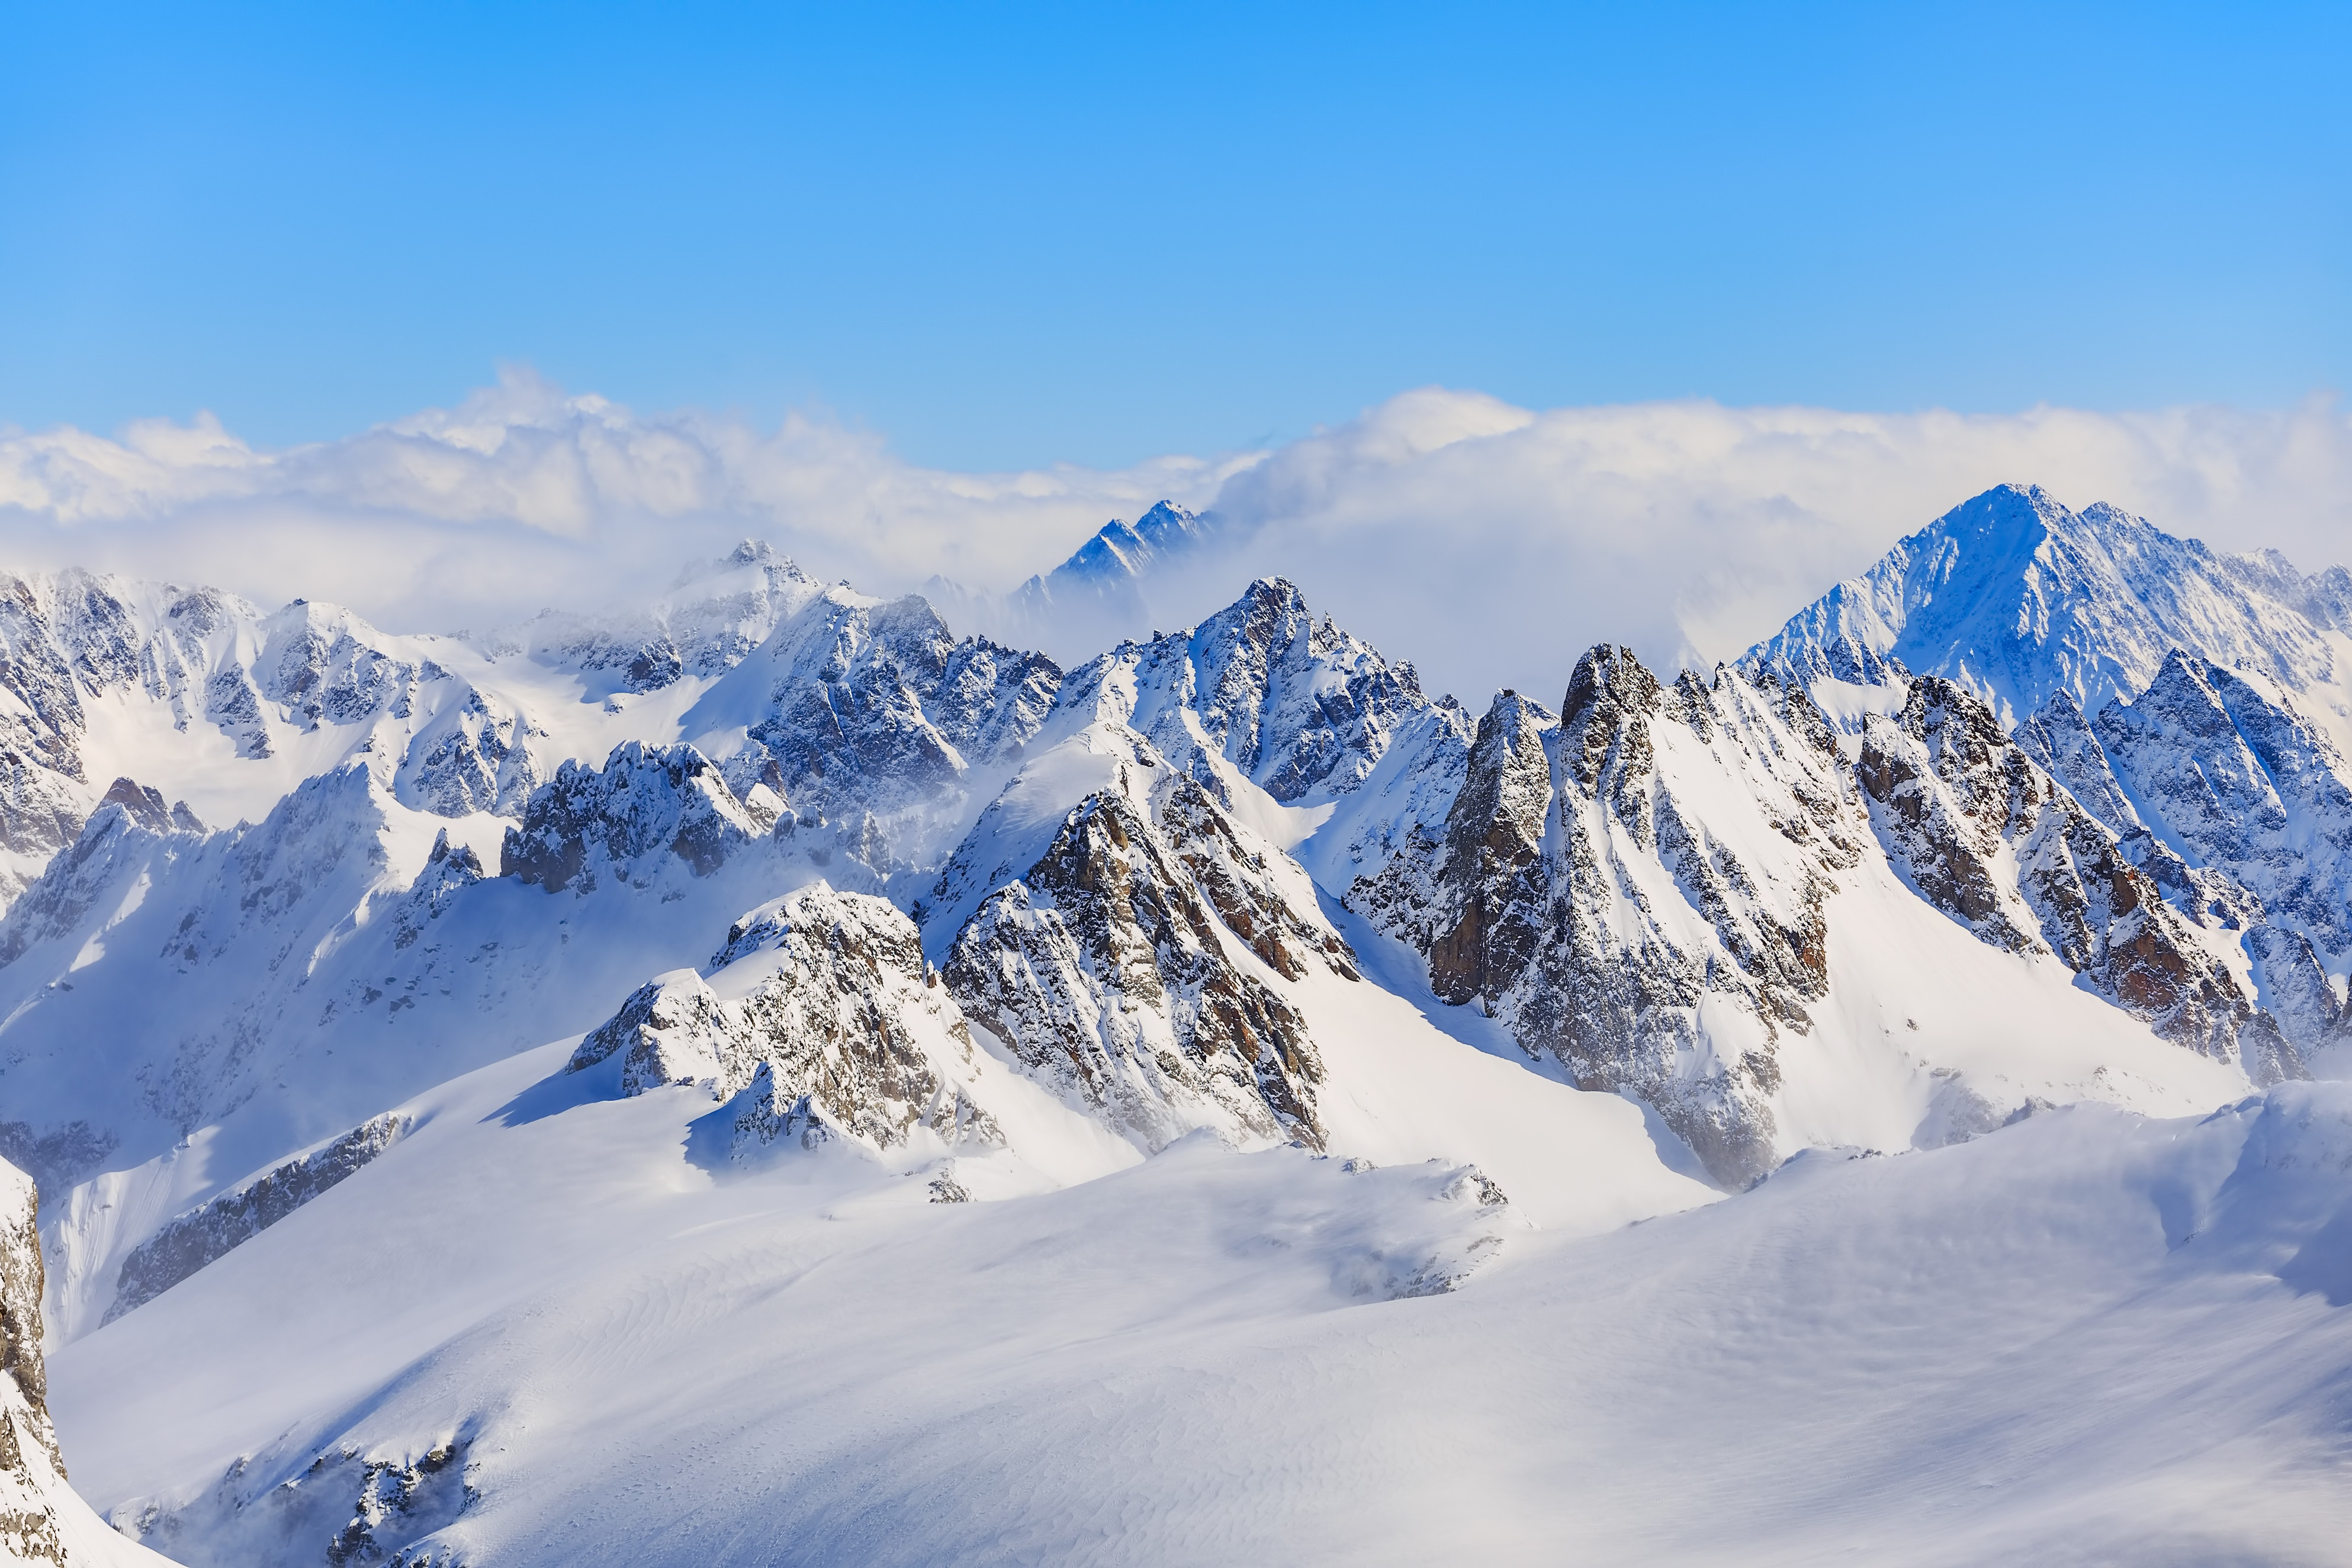
\includegraphics[height=0.1\textheight]{mountain}
    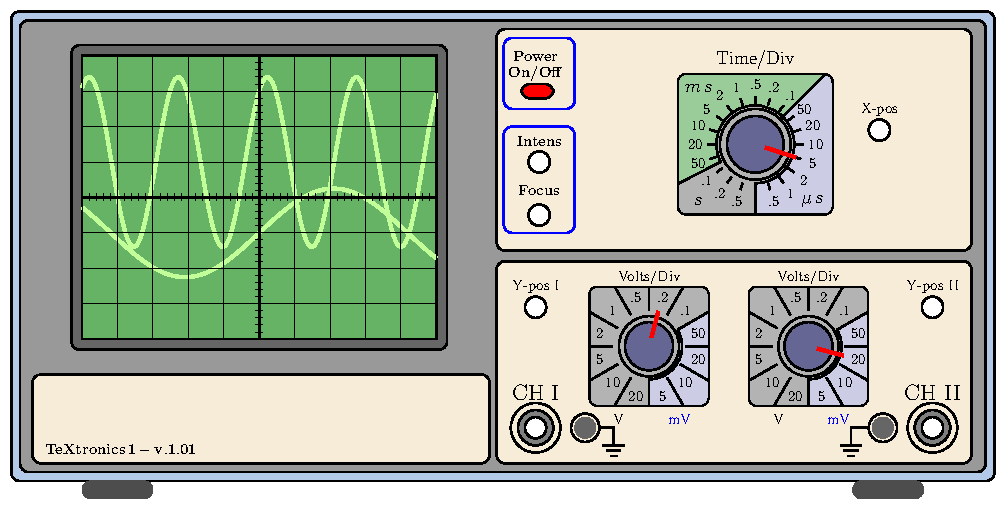
\includegraphics[height=0.1\textheight]{oscilloscope}

    
\includegraphics[width=0.2\textwidth]{lion}
    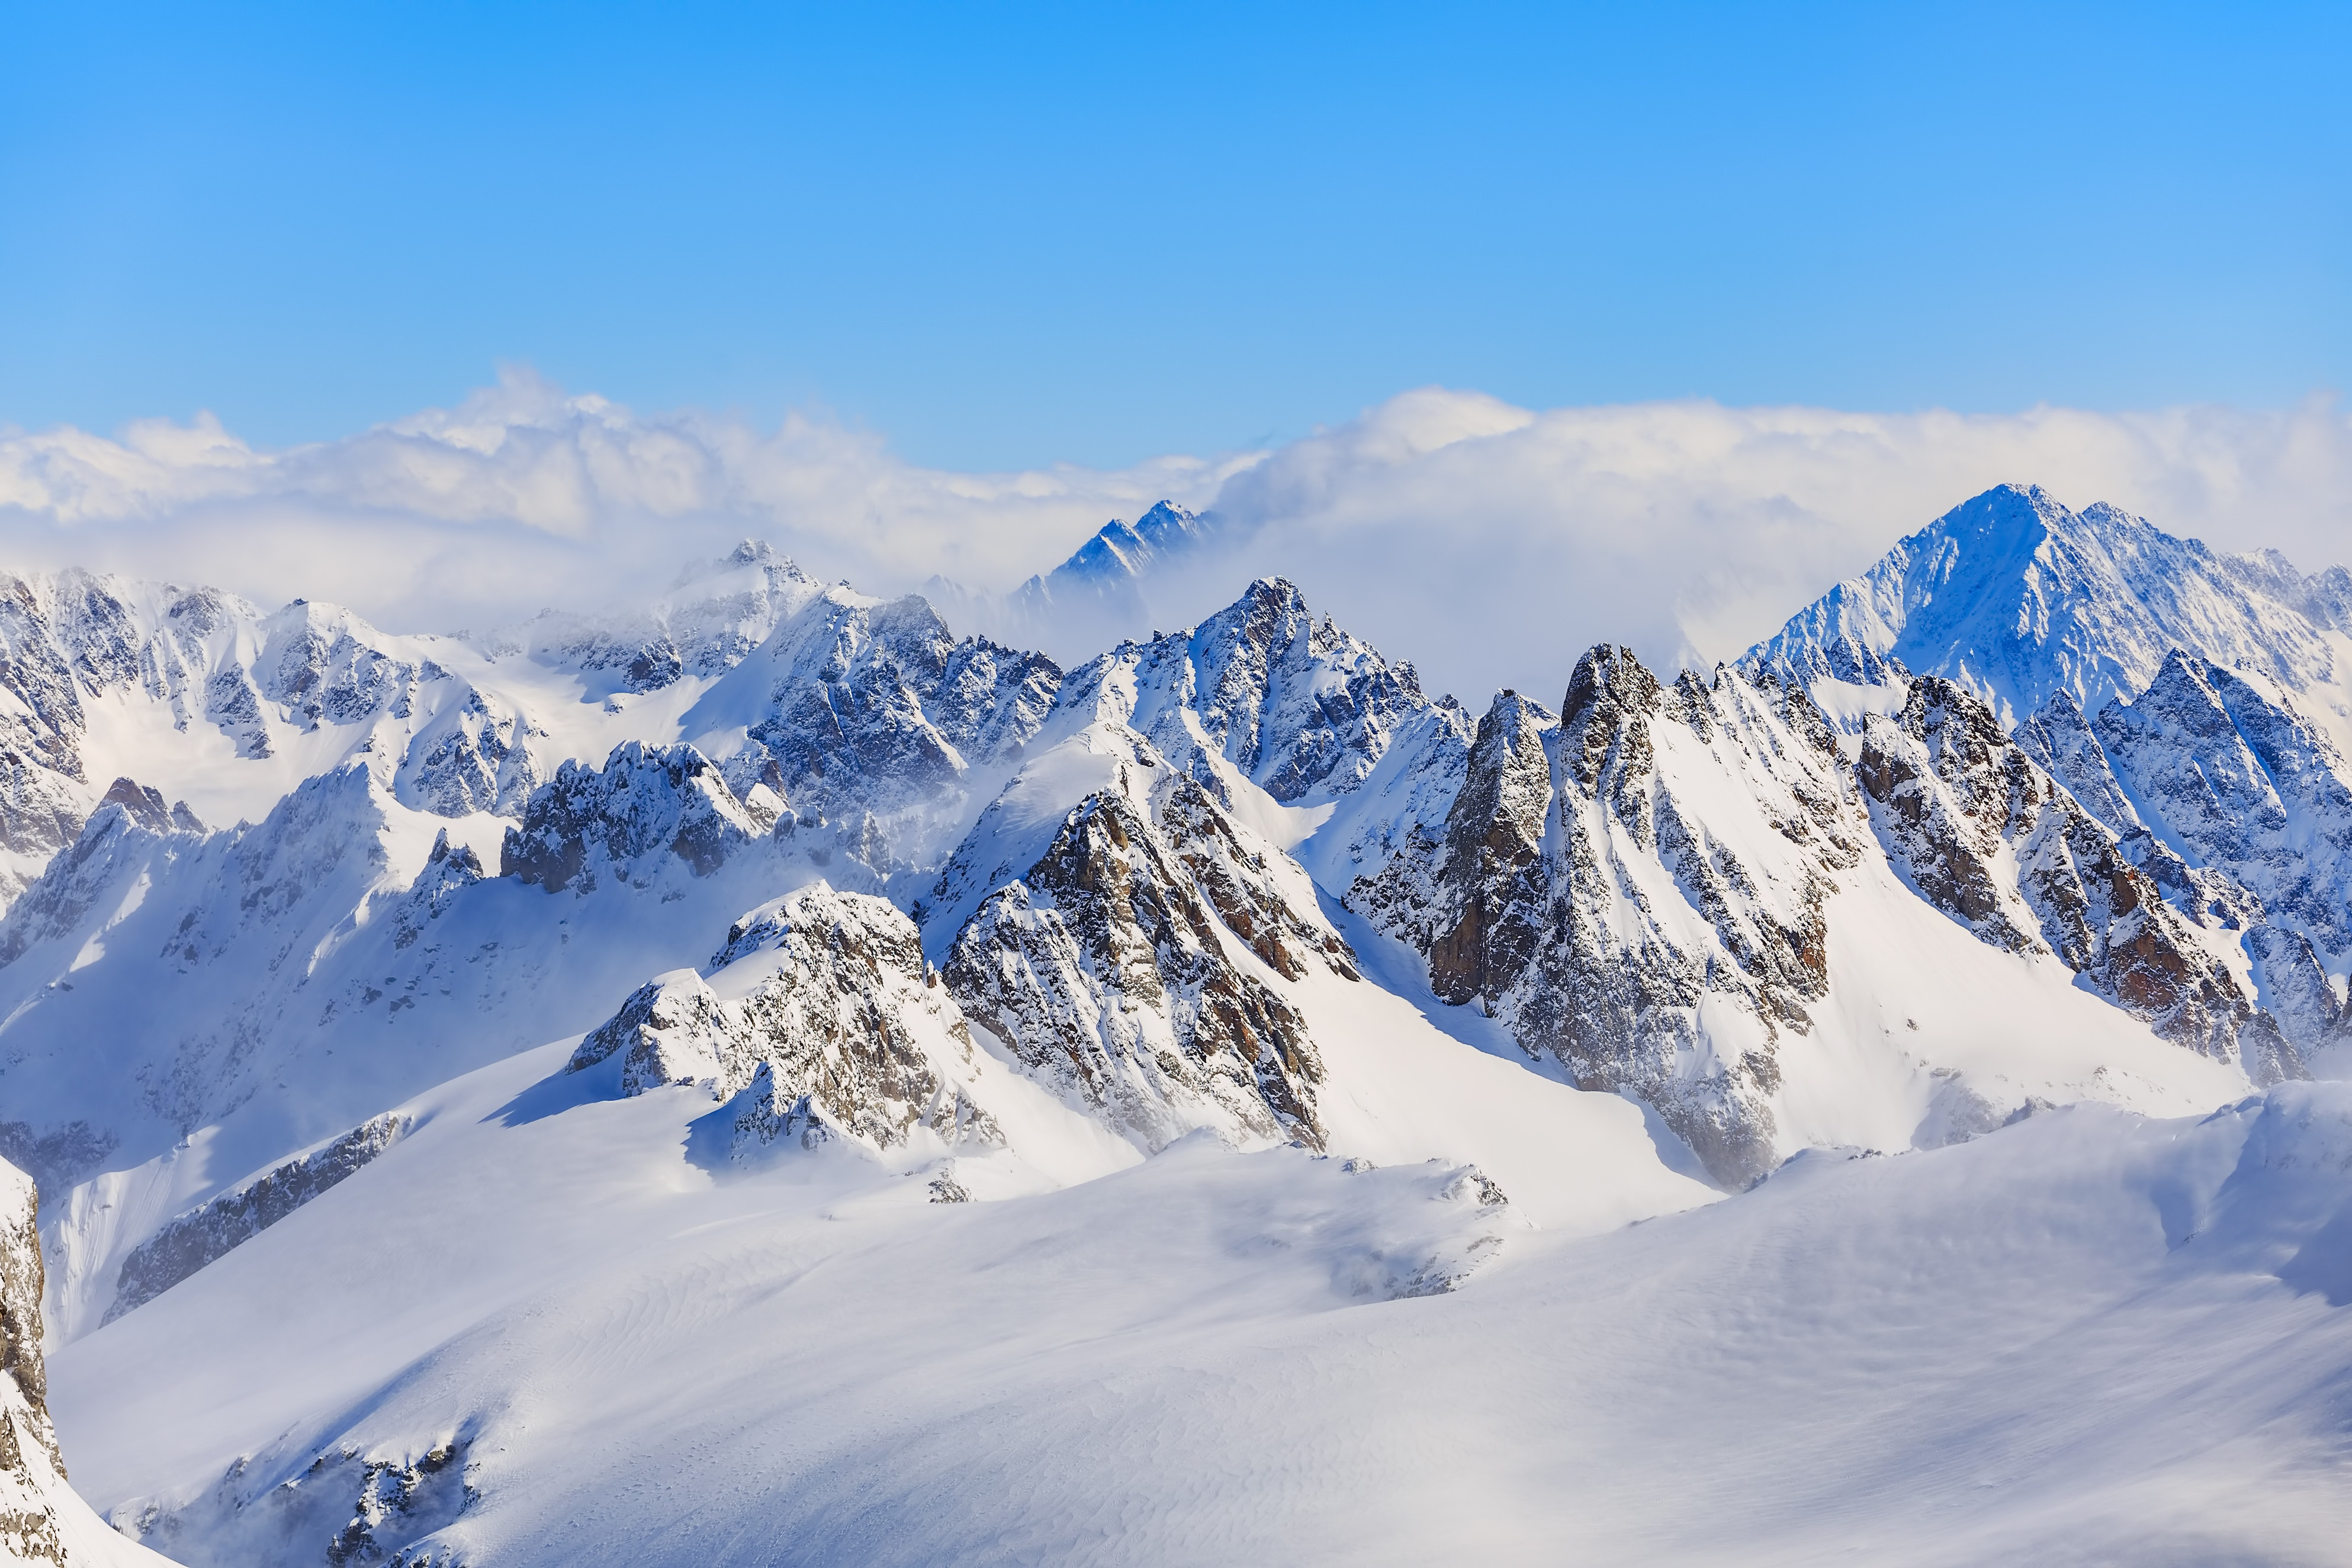
\includegraphics[width=0.2\textwidth]{mountain}
    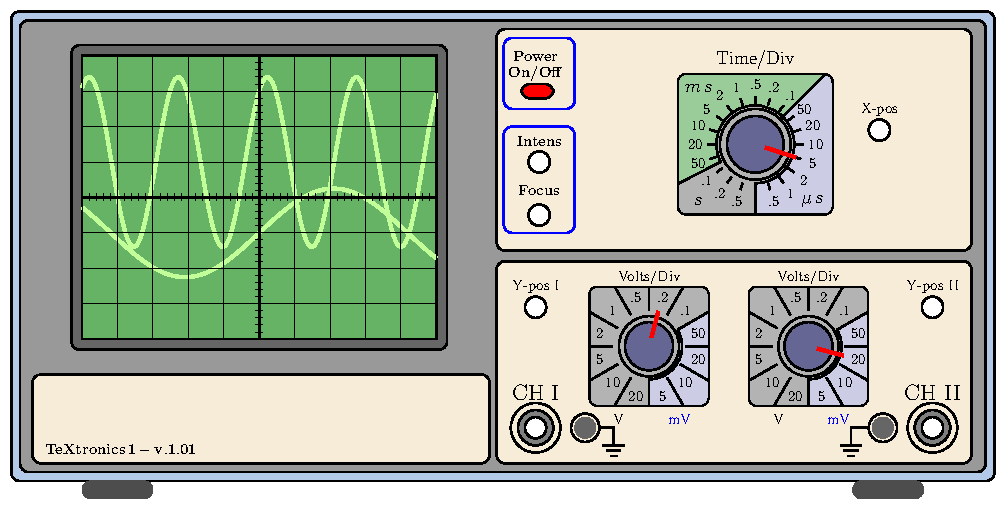
\includegraphics[width=0.2\textwidth]{oscilloscope}

    
\includegraphics[angle=-45,width=0.2\textwidth]{lion}
    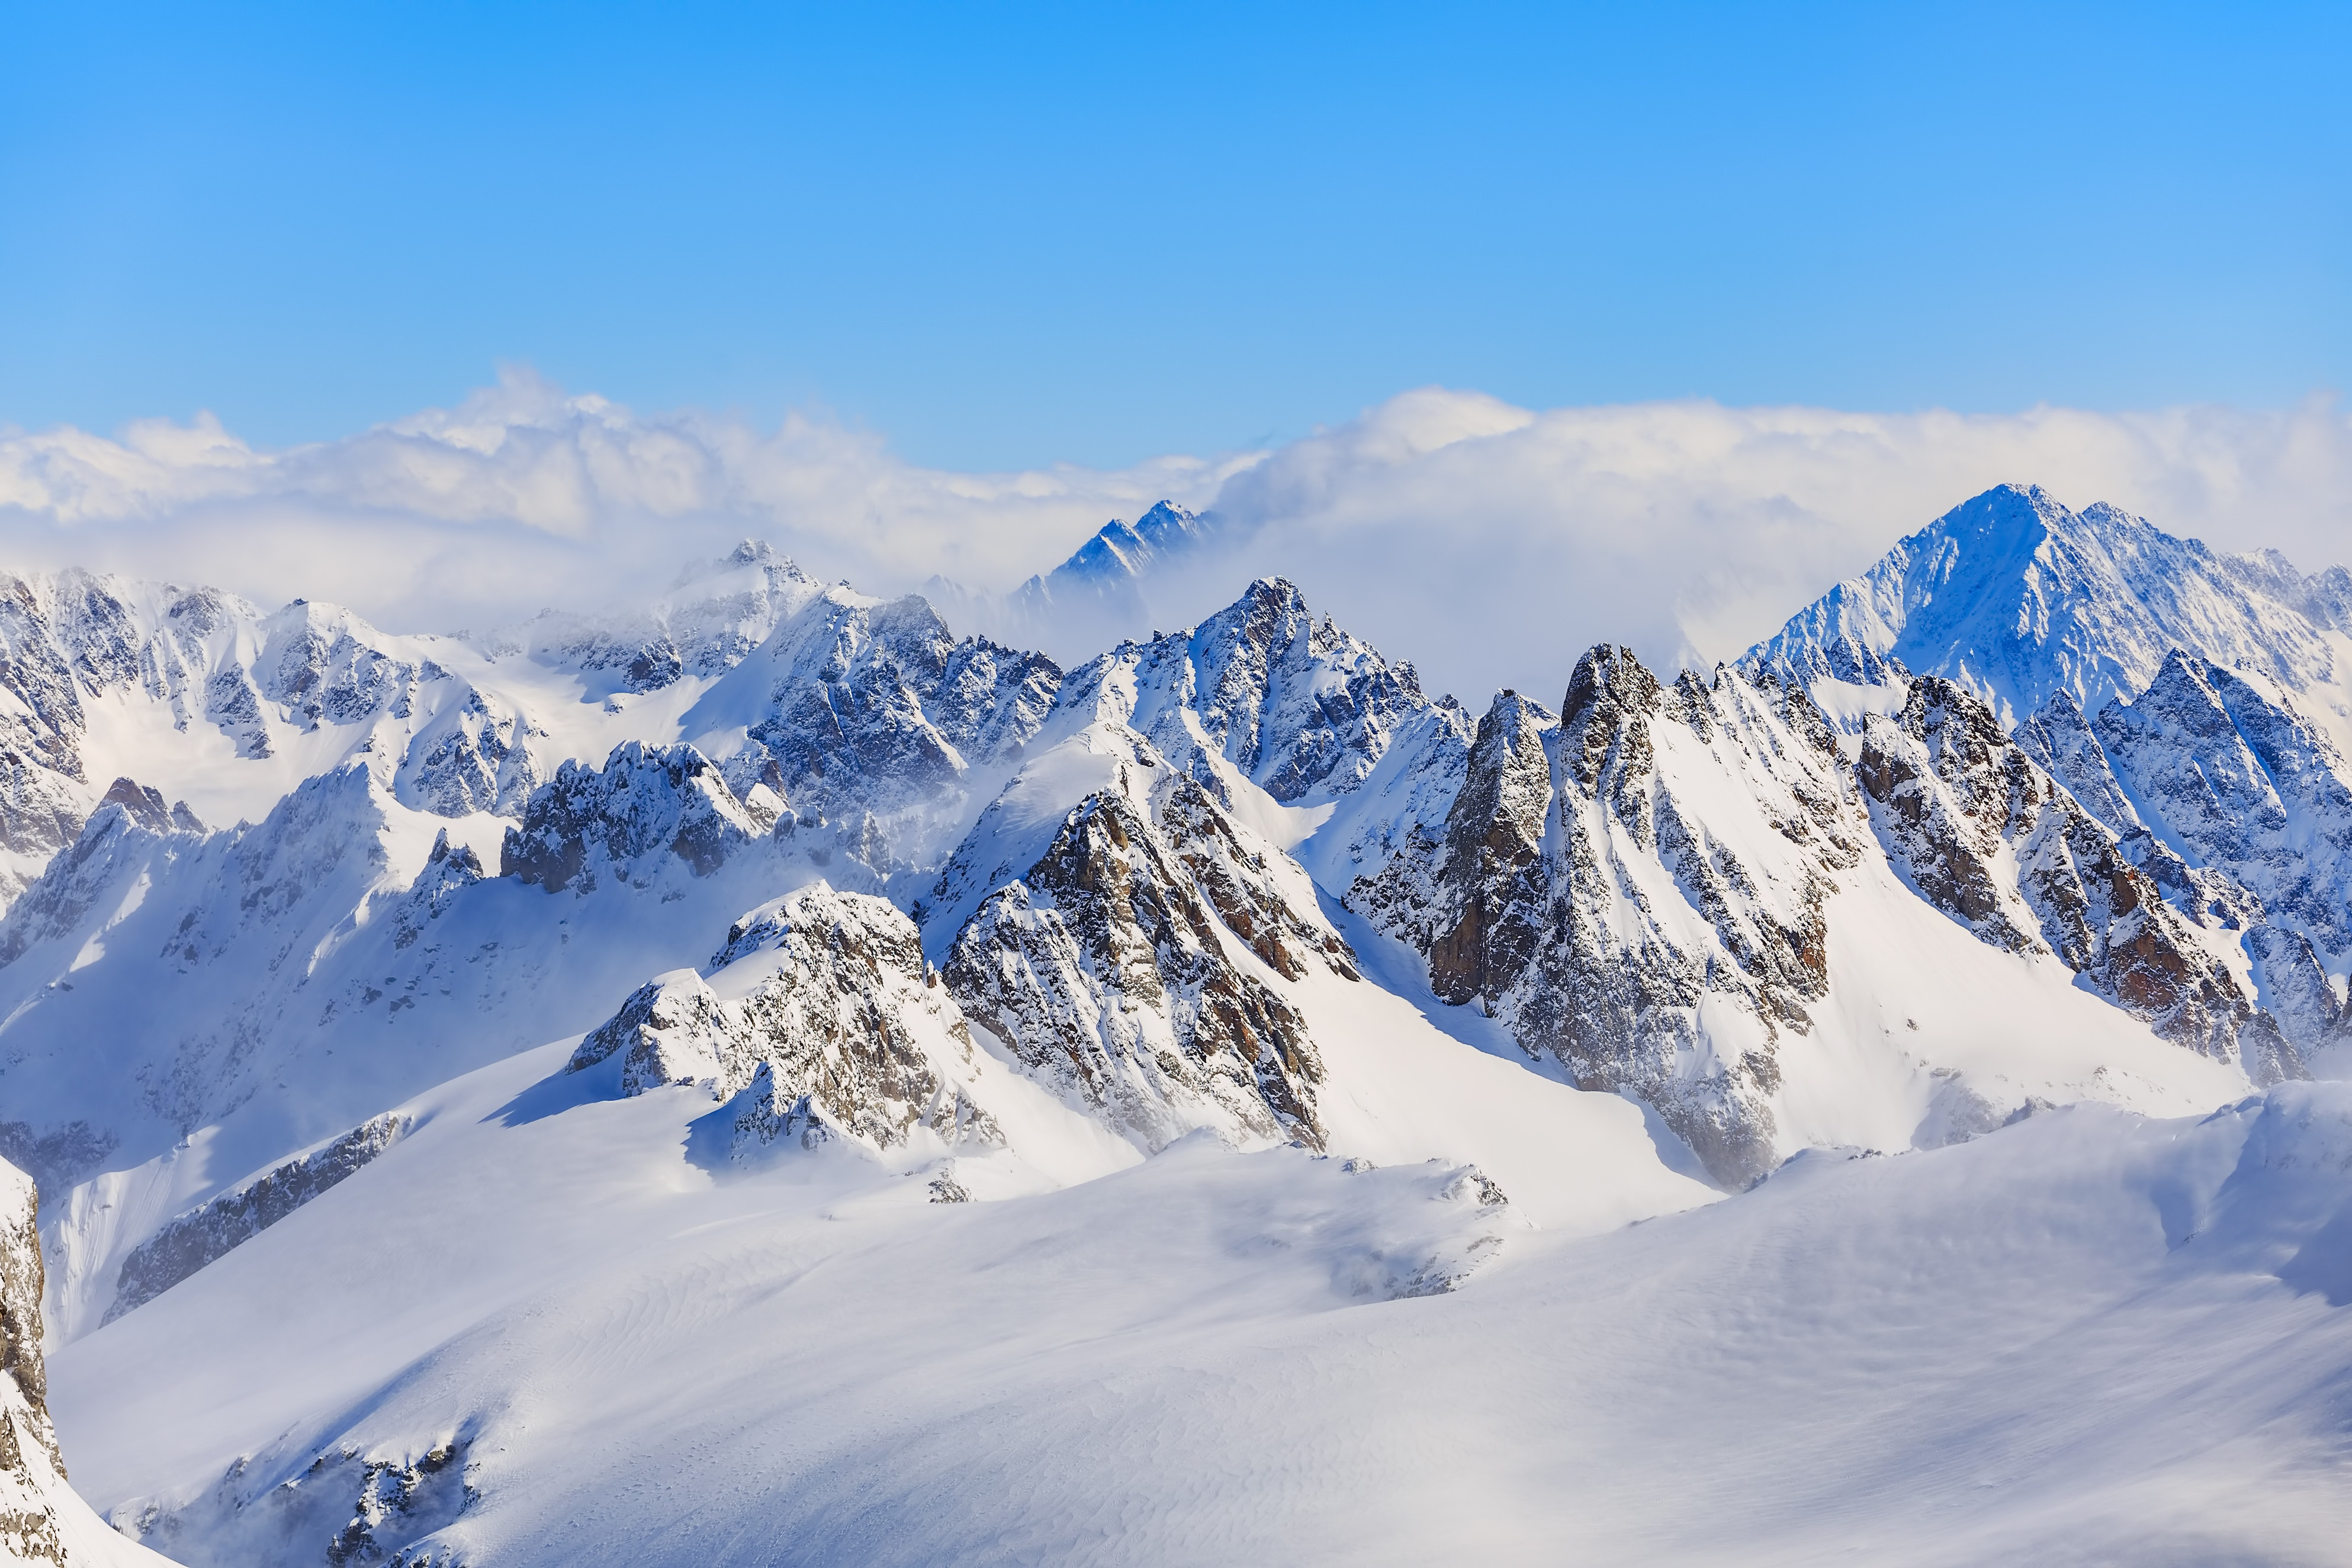
\includegraphics[width=0.2\textwidth]{mountain}
    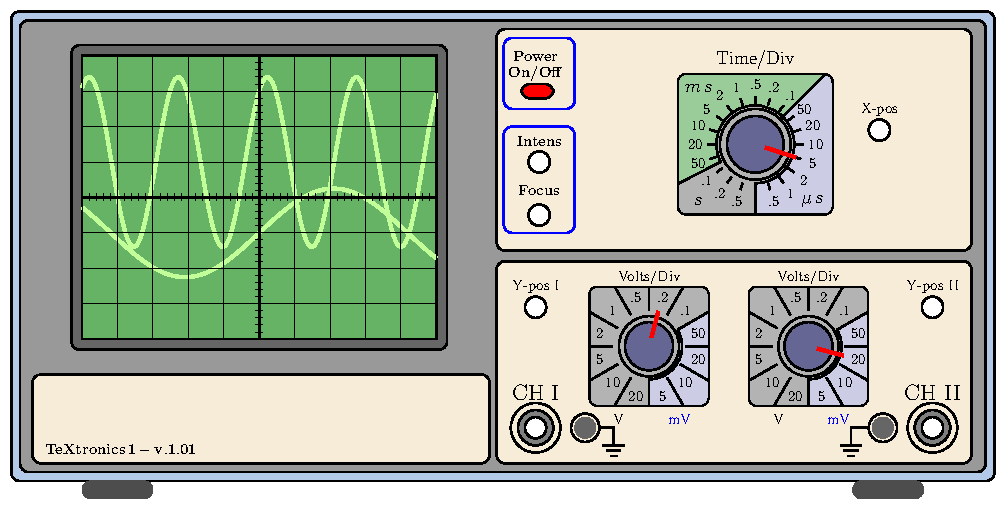
\includegraphics[angle=45,width=0.2\textwidth]{oscilloscope}

    graphicx文档: \href{https://texdoc.net/texmf-dist/doc/latex/graphics/graphicx.pdf}{The graphicx package - graphicx.pdf}

\end{document}